% FROM: https://www.overleaf.com/latex/templates/simple-beamer-theme/cyjyxkdttqzs

\documentclass[aspectratio=169,xcolor=dvipsnames]{beamer}
\usetheme{Simple}

\usepackage{hyperref}
\usepackage{graphicx}
\usepackage{booktabs}
\usepackage{multicol}
\usepackage{tikz}
\usepackage{soul}
\usetikzlibrary{positioning}
\usetikzlibrary{decorations.pathreplacing,calligraphy}

\usepackage[
    backend=bibtex,
    style=authoryear,
    sorting=nyt,
    autocite=inline
]{biblatex}
\addbibresource{references.bib}

\newtheorem{conjecture}{Conjecture}

\graphicspath{ {sections/} }

\newcounter{fig}

%------------------------------------------------
%------------------------------------------------

\title[short title]{Essays in Design Economics \\
                    {\large PhD defense}}
\author[JM] {James Michelson}
\institute[CMU]
{
    Department of Philosophy \\
    Carnegie Mellon University 
    \vskip 3pt
}
\date{July 26, 2024}


\begin{document}


\begin{frame}
    \titlepage
\end{frame}

\begin{frame}{Overview}
    \tableofcontents
\end{frame}

%------------------------------------------------
\section{Preamble}
%------------------------------------------------


\begin{frame}

    \vspace{10mm}
    {\Large{\centerline{Preamble}}}

\end{frame}


% % ----

% \begin{frame}{Structure: Big Picture}

% This thesis answers three interrelated questions:

% \begin{enumerate}
%     \item \textit{`What is the scientific value of economic theory in design economics?'} (Chapter 2)

%     \item \textit{`What is an example of a theoretical contribution in design economics?'} (Chapter 3)

%     \item \textit{`What other problems might this body of theory help with?'} (Chapter 4)
% \end{enumerate}

% \end{frame}


% ----- 


\begin{frame}{What is `Design Economics'?}

Design economics is ``the part of economics intended to further the design and maintenance of markets and other economic institutions'' \autocite[1341]{roth2002}.
\begin{itemize}
    \item Both an collection of institutional design problems and an approach to solving them
\end{itemize}

\vspace{5mm}
Earliest noteworthy success stories are from the 1990s:
\begin{enumerate}
    \item Federal Communication Commission's (FCC) 1994 spectrum auctions
    \item National Residency Matching Program's (NRMP) 1997 residency matching algorithm
\end{enumerate}

\vspace{5mm}
Pioneered the use of experimental and computational methods alongside economic theory

\end{frame}

% ----

\begin{frame}{What is `Design Economics'? II}

Further examples of success:
\begin{itemize}
    \item Electronic marketplaces (Amazon, Uber, AirBnB, etc)
    \item Auction design \autocite{binmore2002, alphabet2024}
    \item Matching new doctors to hospitals \autocite{roth1999}
    \item Kidney exchanges \autocite{roth2007hbs}
    % \item Design of voting rules \autocite{lackner2021}
    % \item Allocating food to food banks \autocite{prendergast2022}
    % \item Data acquisition \& sampling strategies \autocite{roth2012surveys}
    \item ...
\end{itemize}

\vspace{5mm}
Lots of different goals: revenue/welfare maximization, efficiency, stability, etc

\vspace{5mm}
{\color{red}Key idea: design the `rules of the game'}

\end{frame}

% ----

\begin{frame}{What is `Design Economics'? III}

Design economics is also an approach to \textit{doing} economics:
\begin{itemize}
    \item Computation and experiment are ``natural complements'' \autocite[1363]{roth2002} to theory
\end{itemize}

\vspace{5mm}
Parallels drawn with engineering in natural science:

\vspace{2mm}
\begin{quote}
    The simple theoretical model in which the only force is gravity, and beams are perfectly rigid, is elegant and general. But bridge design also concerns metallurgy and soil mechanics, and the sideways forces of water and wind. Many questions concerning these complications can’t be answered analytically but must be explored using physical or computational models. \autocite[1342]{roth2002}
\end{quote}

\end{frame}

% ----

% \begin{frame}{Philosophy, Science, and Philosophy of Science}

% Philosophy of science and ``common sense''
% \begin{itemize}
%     \item (Sorry Dad)
% \end{itemize}

% \vspace{5mm}
% Trade off: abstraction vs recommendation
% \begin{itemize}
%     \item Ultimately, I still harbor scientific aspirations
% \end{itemize}

% \vspace{5mm}
% {\color{red}Conclusion of Chapter 4 falls out of prior philosophical analysis!}

% \end{frame}

% ----



%------------------------------------------------
\section{Economic Theory \& Design Economics}
%------------------------------------------------

\begin{frame}

    \vspace{10mm}
    {\Large{\centerline{Economic Theory \& Design Economics}}}

\end{frame}

% ------

\begin{frame}{The Value of Economic Theory}

What is the value of economic theory in design economics?

\vspace{5mm}
A range of possible views:
\begin{enumerate}
    \item Economic theory is useless (a `collection of fables') \autocite{rubinstein2006,rubinstein2012}
    \item Economic theory sharpens the intutions of economists \autocite{roth2019}
    \item Economic theory has predictive value \autocite{friedman1953}
\end{enumerate}

\vspace{5mm}
{\color{red}My argument: cannot hold (1) in light of successes of design economics}

\end{frame}

% ------

\begin{frame}{The Value of Economic Theory II}

\begin{figure}[H]
    \begin{center}
    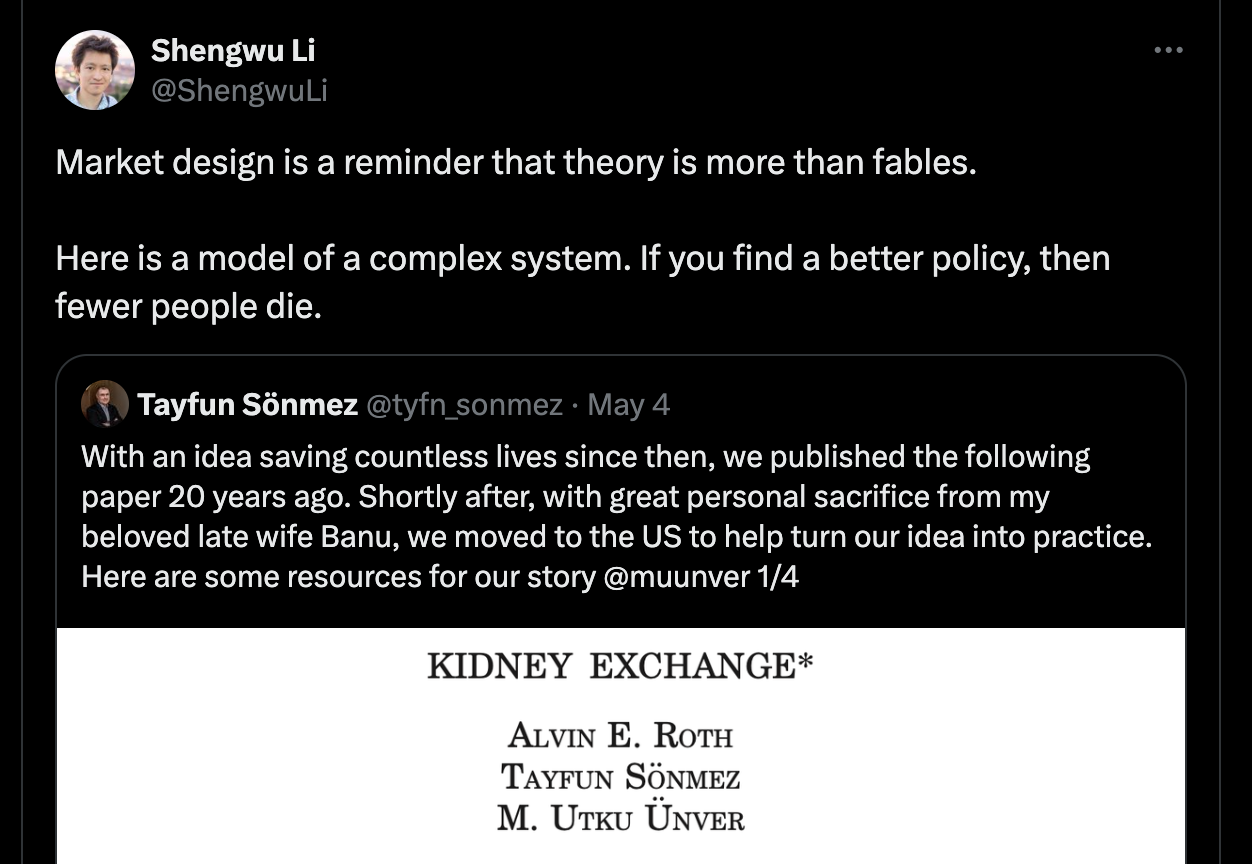
\includegraphics[width=0.65\textwidth]{shengwu_fables.png}
    \end{center}
    
    % \vspace{1mm}
    % \raggedright{\small {\sc Figure \refstepcounter{fig}\thefig\label{fig:pavlov_n2_alloc}:} The allocations produced by the approximation algorithm (left) and exclusive buyer mechanism (right) in the \textbf{symmetric, independent, uniform} case.} 
\end{figure}

\end{frame}

% ------

\begin{frame}{Scientific Success and Philosophy of Science}

\textit{Scientific realism} is the philosophical position that a science's theoretical content is `true'
\begin{itemize}
    \item \textit{scientific anti-realism} is the position that theory is merely a tool
\end{itemize}

\vspace{5mm}
There are \textit{lots} of ways to think about truth

\vspace{5mm}
Realism is most common in the natural sciences (physics)
\begin{itemize}
    \item Argument often follows from observing ``successful'' scientific practices
\end{itemize}

\end{frame}

% ------

\begin{frame}{Scientific Success and The \textit{No-Miracles} Argument}

{\color{red}Key idea: the more successful a science, the more likely its theory is true}

\vspace{5mm}
Structure of the argument:
\begin{align*}
    & P1 \quad \text{Science $X$ is \textit{successful}} \\
    & P2 \quad \text{Science $X$ has theoretical content $Y$} \\
    & P3 \quad \text{If $Y$ weren't \textit{true}, the successes of $X$ would be \textit{miraculous}} \\
    & C1 \quad \text{$Y$ is true}
\end{align*}

Realism ``is the only philosophy that doesn't make the success of science a miracle'' \autocite[73]{putnam1975}

\end{frame}

% ------

\begin{frame}{The \textit{No-Miracles} Argument and Economics}

What about scientific domains where `truth' is a ``non-starter'' \autocite[328]{alexandrova2009}?

\vspace{5mm}
We can adapt the no-miracles argument: what explains a science's succcesses?
\begin{align*}
    & P1 \quad \text{Science $X$ is \textit{successful}} \\
    & P4 \quad \text{Science $X$ has common feature $F$} \\
    & P5 \quad \text{It would be \textit{miraculous} if $F$ didn't explain the success of $X$} \\
    & C2 \quad \text{$F$ explains the success of $X$}
\end{align*}

This project loosely inspired by the idea of \textit{local realism} \autocite{maki2009}

\end{frame}

% ------

% \begin{frame}{The Successes of Design Economics}

% (See Section 2.3 ...)

% \vspace{5mm}
% \begin{itemize}
%     \item FCC spectrum auctions (1994)
%     \item Residency matching (1996)
%     \item British 3G telecom licenses (2000)
%     \item Boston public school choice (2000s)
%     \item Kidney exchanges (2000s)
%     \item Google's online ad auctions (ongoing)
% \end{itemize}

% \vspace{5mm}
% {\color{red}Lots of different goals: revenue-maximization, welfare-maximization, effeciency, stability, equity, etc.}

% \end{frame}

% ------

\begin{frame}{What Explains This Success?}

I consider two principal features:
\begin{enumerate}
    \item Experiment \& computation
    \item Theory
\end{enumerate}

\vspace{5mm}
Everyone (?) agrees (1) experiment and computation matter

\vspace{5mm}
Big disagreements about the value of economic theory

\end{frame}

% ------
\begin{frame}{A \textit{Minimal Non-Fable} Account of the Value of Theory}

\vspace{5mm}
Succeses have already been established ($P1$); need to show there are common theoretical features ($P4$) that are \textit{non-arbitrary} ($P5$)

\vspace{5mm}
Game theory is likely common to all the successes above (theoertical overlap)

\vspace{5mm}
Economic theory in design economics is \textit{projective} \autocite{guala2001}
\begin{itemize}
    \item Theory models decisions economists and policymakers subsequently take
\end{itemize}


\end{frame}



% ------

% \begin{frame}{A \textit{Minimal Non-Fable} Account of the Value of Theory}

% {\color{red}Economic theory ought ``not aspire toward purposefulness... [and] does not engage in predictions and recommendations'' \autocite[35-6]{rubinstein2012}}

% \vspace{5mm}
% Succeses have already been established ($P1$); need to show there are common theoretical features ($P4$) that are \textit{non-arbitrary} ($P5$)

% \vspace{5mm}
% Game theory is likely common to all the successes above (theoertical overlap)

% \end{frame}


% ------

% \begin{frame}{A \textit{Minimal Non-Fable} Account of the Value of Theory II}

% Economic theory in design economics is \textit{projective} \autocite{guala2001}

% \vspace{5mm}
% Theory models decisions economists and policymakers subsequently take
% \begin{itemize}
%     \item The world can be made to ``mirror'' the model
%     \item This ``mirroring'' can be made arbitrary close (e.g., online ad auctions)
% \end{itemize}

% \vspace{5mm}
% {\color{red}Key idea: economic theory in this domain models the part of the world it changes}

% \end{frame}

% ------

\begin{frame}{Conclusion}

\vspace{5mm}
Game theory is the common theoretical feature shared by the success stories of design economics

\vspace{5mm}
Modeling the control we exert in a model minimizes the ``gap'' between representation and reality

\vspace{5mm}
{\color{red}$\implies$ Economic theory partly explains the success of design economics}

% \vspace{5mm}
% \begin{quote}
%     If I had to name one major shift in the sensibilities of economic theorists in the past half century, a prime candidate would be the way we conceptualize markets---from quasi-natural phenomena admired from afar to man-made institutions whose design can be tweaked by economist-engineers. \autocite[p137]{spiegler2024}
% \end{quote}


\end{frame}



%------------------------------------------------
\section{Optimal Multidimensional Auction Design}
%------------------------------------------------


\begin{frame}

    \vspace{10mm}
    {\Large{\centerline{Optimal Multidimensional Auction Design}}}

\end{frame}

% ------

\begin{frame}{The Problem}

Among all possible ways of selling a single good with multiple quality levels, which should a seller use if they want to maximize their profits?

\vspace{5mm}
\begin{itemize}
    \item $K\geq1$ `quality levels'
    \item $N\geq1$ bidders
    \item Assume: bidders are risk neutral with i.i.d. valuations
\end{itemize}

\vspace{5mm}
Example: buying a radio spectrum license from the government (duration, coverage, use, etc)

\end{frame}

% ------


\begin{frame}{Approach}

{\color{red}Problem: analytically intractable setting!}

\vspace{5mm}
Use simulations to understand the qualitative features of the optimal auction

\vspace{5mm}
Compare approximately optimal mechanism yielded by the algorithm to prior conjecture
\begin{itemize}
    \item Lots of different settings!
\end{itemize}

\end{frame}

% ------

\begin{frame}{The \textit{exclusive-buyer mechanism}}

Key idea: buyers compete for the right to be the only buyer, and then choose which quality level to purchase. 
\begin{itemize}
    \item Competition = second price or ascending-bid auction
\end{itemize}

\vspace{5mm}
Allocate the good according to the maximum of bidders' quality grade-specific virtual values $\beta^i = \max_{j'} \beta_{j'}^i$

\vspace{5mm}
I investigate the specific case of linear virtual values $\beta_j^i = x_j^i - r_j$, where $r_j$ is the \textit{reserve price}

\end{frame}

% ------ 

\begin{frame}{Conjectures (Auction Design)}

\vspace{5mm}
\begin{conjecture}[Revenue]\label{conj_rev}
The revenue of the exclusive buyer mechanism well-approximates the revenue of the optimal mechanism.
\end{conjecture}

\vspace{5mm}
\begin{conjecture}[Allocations]\label{conj_alloc}
The allocation of the exclusive buyer mechanism well-approximates the allocation of the optimal mechanism yielded by the approximation algorithm.
\end{conjecture}

\end{frame}

% ------ 

\begin{frame}{Conjectures (Exclusion)}

\vspace{5mm}
\begin{conjecture}[Measure Zero Exclusion Region]\label{conj_excl_zero}
There exist multidimensional settings where a single good with multiple quality levels is sold to multiple bidders with a measure zero exclusion region.
\end{conjecture}

\vspace{5mm}
\begin{conjecture}[Same Exclusion Region for all $N$]\label{conj_excl_n}
The exclusion region of the optimal mechanism in the multidimensional setting of a single good with multiple quality levels remains the same for $N=1,2,3,\dots$ bidders. 
\end{conjecture}

\end{frame}

% ------ 

\begin{frame}{Results: Conjecture (Revenue)}

\textbf{This conjecture is supported in all settings}

\vspace{5mm}
However, it is known that simple (deterministic) mechanisms can well-approximate optimal (stochastic) mechanisms up to some constant fraction of their value.

\vspace{5mm}
The gain from using the optimal mechanism over the best deterministic mechanism is typically $\sim$1-2\% in instances where randomization is required for optimality

\vspace{5mm}
{\color{red} Surprisingly, deterministic mechanisms are sometimes optimal!}

\end{frame}

% ------ 

\begin{frame}{Results: Conjecture (Allocations)}

\begin{figure}[H]
    \begin{center}
    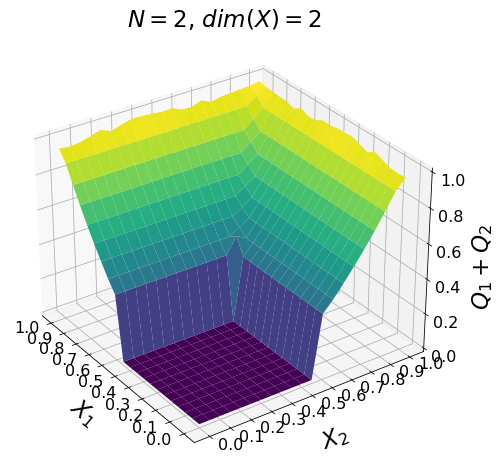
\includegraphics[width=0.45\textwidth]{images/symmetric_independent_unif_01.png}
    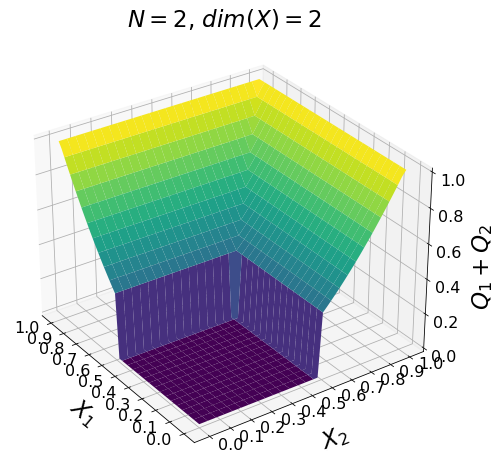
\includegraphics[width=0.44\textwidth]{images/symmetric_independent_unif_01_ebm.png}
    \end{center}
    
    \vspace{1mm}
    \raggedright{\small {\sc Figure \refstepcounter{fig}\thefig\label{fig:pavlov_n2_alloc}:} The allocations produced by the approximation algorithm (left) and exclusive buyer mechanism (right) in the \textbf{symmetric, independent, uniform} case.} 
\end{figure}

\end{frame}

% -------

\begin{frame}{Results: Conjecture (Allocations) II}

\textbf{This conjecture is supported when there is no evidence of randomization in the optimal mechanism}
\begin{itemize}
    \item Problem cases: symmetric, independent, uniform \autocite{pavlov2011optimal} and asymmetric, independent, uniform \autocite{belloni2010multidimensional}
\end{itemize}

\vspace{5mm}
Allocations are qualitatively \textit{very} similar in many settings

\vspace{5mm}
{\color{red}Suggests major issue lies in identifying when randomization is required; when it is not, exclusive-buyer mechanism likely optimal!}



\end{frame}


% ------ 

\begin{frame}{Results: Conjecture (Measure Zero Exclusion Region)}

\textbf{This conjecture is only supported in the asymmetric, independent, uniform setting}
\begin{itemize}
    \item $X_1 \sim U[6,8]$, $X_2 \sim U[9,11]$, $c_1 = .9, c_2 = 5$ \autocite{belloni2010multidimensional}
\end{itemize}

\vspace{5mm}
This stands in contrast to theoretical work in the related multi-unit setting, which shows that it is always optimal to exclude a positive measure of buyers \autocite{armstrong1996multiproduct,rochet1998ironing}


\end{frame}

% ------ 

\begin{frame}{Results: Conjecture (Same Exclusion Region for all $N$)}

\textbf{This conjecture is supported in all settings}
\begin{itemize}
    \item For cases $N=1,2,3$
\end{itemize}

\vspace{5mm}
Suggests that $N=1$ results can be used as `stepping-stone' for $N>1$ investigations, as in the case of \autocite{pavlov2011optimal} (above)

\end{frame}

% ------ 

\begin{frame}{Conclusion}

Exclusive-buyer mechanism is often optimal!
\begin{itemize}
    \item Depends on whether randomization is required for optimality
\end{itemize}

\vspace{5mm}
Future work:
\begin{itemize}
    \item \textit{stochastic} exclusive-buyer mechanism
    \item non-linear virtual values $\beta_j^i$
\end{itemize}

\end{frame}





%------------------------------------------------
\section{Reflexive Measurement}
%------------------------------------------------

\begin{frame}

    \vspace{10mm}
    {\Large{\centerline{Reflexive Measurement}}}

\end{frame}

% -------

\begin{frame}{The Causal Effects of Science Itself}

Scientific practices can interfere with their targets of investigation

\vspace{5mm}
Example: bank runs
\begin{itemize}
    \item Predicting a bank run can cause/exacerbate one!
\end{itemize}

\vspace{5mm}
Example: psychology experiments
\begin{itemize}
    \item Study particants often guess what the experiment wants!
\end{itemize}

\vspace{5mm}
{\color{red}Goal: give a general account of this phenomenon}

\end{frame}

% -------

\begin{frame}{Jargon}

Social science/philosophy
\begin{itemize}
    \item ``Self-fulfilling science'' \autocite{merton1948} \textbf{(Sociology, Economics)}
    \item ``Performativity'' \autocite{healy2015} \textbf{(Sociology)}
    \item ``Non-oxymoron criterion'' \autocite{luce95} \textbf{(Psychology)}
    \item ``Reflexive prediction'' \autocite{buck1963} \textbf{(Philosophy)}
    \item ``Looping effects'' \autocite{hacking1983} \textbf{(Philosophy)}
    \item ``Reactivity'' \autocite{runhardt2023} \textbf{(Philosophy, Sociology?)}
    \item ``Oedipus effect'' \autocite{popper1953} \textbf{(Philosophy)}
    \item ``Goodhart's Law'' \autocite{goodhart1984} \textbf{(Economics)}
\end{itemize}

\vspace{5mm}
Stats/CS
\begin{itemize}
    \item ``Performative prediction'' \autocite{perdomo2020} \textbf{(CS)}
    \item ``Strategic classification'' \autocite{hardt2016} \textbf{(CS)}
    \item ``Incentive compatible learning'' \autocite{dekel2010} \textbf{(CS)}
    \item ``Statistical contract theory'' \autocite{bates2022} \textbf{(CS)}
\end{itemize}

\end{frame}



% -------

% \begin{frame}{Reflexivity \& Philosophy of Science}

% % Old idea: ``complicated interaction between observer and observed'' \autocite[14]{popper1953}

% Overwhelmingly concerned with the role of predictions on changing predicted events

% \vspace{5mm}
% Early focus was on `formulation and dissemination style' \autocite{romanos1973}
% \begin{itemize}
%     \item Causal effect of prediction depends on how it is given
% \end{itemize}

% \vspace{5mm}
% Two big recent developments:
% \begin{itemize}
%     \item \textit{Probabilitistic} account of reflexive predictions \autocite{kopec2011}
%     \item Degrees of reflexivity \autocite{lowe2018,cejka2022}
% \end{itemize}



% \end{frame}


% % -------

% \begin{frame}{Reflexivity \& Economics}


% Oskar Morgenstern (1928) \textit{Wirtschaftsprognose: Eine Untersuchung Ihrer Voraussetzungen und Möglichkeiten}\footnote{Most promisingly translated as: \textit{Economic Forecasting: A Study of its Conditions and Possibilities}}
% \begin{itemize}
%     \item Investigates self-defeating predictions in business cycle theory
%     \item Problem: the attempt to make a correct public prediction by taking into account the agents' reaction to it leads to an infinite regress
% \end{itemize}

% % \vspace{5mm}
% % {\color{red}``... ``purely statistical'' considerations can never satisfy as a means of explanation and so ultimately of forecast.'' \autocite[319]{marget1929}}

% \vspace{5mm}
% More recently: reflexivity and complex systems \autocite{soros2013, beinhocker2013}


% \end{frame}


% % -------

% \begin{frame}{Reflexivity \& Psychology}

% Experimental psychology has a long history of confronting reflexivity as a practical challenge
% \begin{itemize}
%     \item `Experimenter effect' \autocite{rosenthal1966}, `Demand characteristics' \autocite{orne1962}, `Pygmalion effect' \autocite{rosenthal1968}, etc
% \end{itemize}

% \vspace{5mm}
% Developed \textit{non-oxymoron criterion} \autocite{luce95}
% \begin{itemize}
%     \item Psychological hypotheses should not be able to be discomfirmed `at will'
%     \item $\implies$ Design studies so as it ``behooves the subejcts to reveal their true preferences'' \autocite[9]{luce95}
% \end{itemize}

% \end{frame}


% -------

\begin{frame}{What is Reflexivity? (My Proposal)}

Focus on sociological account of scientific practice
\begin{itemize}
    \item What is it that scientists actually \textit{do}?
\end{itemize}

\vspace{5mm}
Don't want to narrowly focus on prediction, measurement, etc

\vspace{5mm}
Consequence: broaden scope to consider \textit{collateral effects}
\begin{itemize}
    \item Google's `Don't Be Evil' motto \autocite{basu2015}
\end{itemize}


\end{frame}

% -------

\begin{frame}{What is Reflexivity? (My Proposal) II}

{\color{red}What matters is people's \textit{awareness} of their part in a \textit{scientific investigation}}
\begin{itemize}
    \item Generalizes the notion of ``partial belief'' in reflexive prediction \autocite[484]{grunberg1986}
\end{itemize}

\vspace{5mm}
This is a broad definition! 
\begin{itemize}
    \item Avoids focus on reflexive effects (changes in outcome, changes in probability, etc)
    \item Relevant causal pathway for these affects is agent's awareness
\end{itemize}

\vspace{5mm}
This is a necessary \textit{but not sufficient} condition
\begin{itemize}
    \item Ask me about aliens...
\end{itemize}

\end{frame}


% ----- 

\begin{frame}{Reflexive Measurement}

{\color{red}Key idea: `measurement as intervention' \autocite{morgan2001}}

\vspace{5mm}
\begin{quote}     
    ``The ways in which the economic body is investigated and data are collected, categorized, analyzed, reduced, and reassembled amount to a set of experimental interventions---not in the economic process itself, but rather in the information collected from that process.`` \autocite[p237]{morgan2001}
\end{quote}

\vspace{5mm}
Helpful to consider the distinction between \textit{data} and \textit{phenomena} \autocite{woodward1989}
\begin{itemize}
    \item Scientists can affect the underlying measurement construct (Stanford Prison Experiment)
    \item Or just change the incentives so people will lie (Surveys)
\end{itemize}

\end{frame}


% ----- 

\begin{frame}{Reflexive Measurement \& Distribution Shift}

How to understand the problem of mis-aligned incentives in reflexive measurement?

\vspace{5mm}
De-biasing systematic component of measurement error does not work
\begin{itemize}
    \item Narrow focus on first moment of distribution
    \item Assumes distribution itself doesn't change
\end{itemize}

\vspace{5mm}
{\color{red}A problem of \textit{distribution shift}: the sample distribution no longer accurately reflects the population data model}

\end{frame}

% ----- 

\begin{frame}{Incentive-Compatible Measurement}

{\color{red}Goal: design measurements that are incentive-compatible!}
\begin{itemize}
    \item Remove the incentive to lie / misreport results
\end{itemize}

\vspace{5mm}
It turns out there's a related literature in theoretical computer science!
\begin{itemize}
    \item Related to work in \textit{performative prediction} \autocite{perdomo2020,oesterheld23}
\end{itemize}

\vspace{5mm}
Application of economic theory to measurement problems
\begin{itemize}
    \item Arguments in Chapter 2 apply!
\end{itemize}

\end{frame}


% ----- 

\begin{frame}{Conclusion}

Reflexivity is general property of science
\begin{itemize}
    \item What matters is when people are aware of their status as objects of inquiry
\end{itemize}

\vspace{5mm}
In the context of measurement, this is akin to the idea of `measurement as intervention' \autocite{morgan2001}

\vspace{5mm}
This problem is best characterized as a problem of distribution shift
\begin{itemize}
    \item Explicitly accounting for the incentives is a promising way to address this \autocite{luce95}
\end{itemize}

\vspace{5mm}
{\color{red}$\implies$ build telescopes!}

\end{frame}






%------------------------------------------------
\section{Conclusion}
%------------------------------------------------

\begin{frame}

    \vspace{10mm}
    {\Large{\centerline{Conclusion}}}

\end{frame}

\begin{frame}{Conclusing Remarks}

Theory matters for design!

\vspace{5mm}
Sometimes simple mechanisms are optimal in complex settings!

\vspace{5mm}
Design incentive-compatible measurements!

\end{frame}



\begin{frame}

    \vspace{10mm}
    {\Large{\centerline{Thank you for listening!}}}

\end{frame}




\begin{frame}

    \vspace{10mm}
    {\Large{\centerline{Bonus Slides}}}

\end{frame}

\begin{frame}{Settings}

\begin{itemize}
    \item \textbf{Symmetric, independent, uniform}: $X_1,X_2 \sim U[0,1]$ and $X_1,X_2 \sim U[2,3]$ \autocite{pavlov2011optimal}
    \item \textbf{Symmetric, independent, non-uniform}: $X_1,X_2 \sim Beta(\alpha,\beta)$ with $\alpha=1, \beta=2$ \autocite{daskalakis2017strong}
    \item \textbf{Symmetric, correlated}: $X_1 = X_2 = [0,1]$, $f(x_1,x_2) = x_1 + x_2$
    \item \textbf{Asymmetric, independent, uniform}: $X_1 \sim U[6,8]$, $X_2 \sim U[9,11]$, $c_1 = .9, c_2 = 5$ \autocite{belloni2010multidimensional}
    \item \textbf{Asymmetric, independent, non-uniform}: $X_1 \sim truncnorm(\mu=2.3,\sigma=1,\underline{x}_1=2,\overline{x}_1=3)$, $X_2 \sim truncnorm(\mu=2.8,\sigma=.2,\underline{x}_1=2,\overline{x}_1=3)$
\end{itemize}

\end{frame}



% \begin{frame}{Jargon}

% Stats/CS/economics
% \begin{itemize}
%     \item ``Performative prediction'' \autocite{perdomo2020} \textbf{(CS)}
%     \item ``Strategic classification'' \autocite{hardt2016} \textbf{(CS)}
%     \item ``Incentive compatible learning'' \autocite{dekel2010} \textbf{(CS)}
%     \item ``Incentive compatible estimation'' \autocite{eliaz2022} \textbf{(Economics)}
%     \item ``Statistical contract theory'' \autocite{bates2022} \textbf{(CS)}
% \end{itemize}

% \vspace{5mm}
% Social sciences/philosophy of science
% \begin{itemize}
%     \item ``Self-fulfilling science'' \autocite{merton1948} \textbf{(Sociology, Economics)}
%     \item ``Performativity'' \autocite{healy2015} \textbf{(Sociology)}
%     \item ``Non-oxymoron criterion'' \autocite{luce95} \textbf{(Psychology)}
%     \item ``Reflexive prediction'' \autocite{buck1963} \textbf{(Philosophy)}
%     \item ``Looping effects'' \autocite{hacking1983} \textbf{(Philosophy)}
%     \item ``Reactivity'' \autocite{runhardt2023} \textbf{(Philosophy, Sociology?)}
%     \item ``Oedipus effect'' \autocite{popper1953} \textbf{(Philosophy)}
% \end{itemize}

% \end{frame}



% \begin{frame}
%     \vspace{10mm}
%     \centerline{\Huge Performative Prediction}
% \end{frame}

% %------------------------------------------------
% \subsection{Model \& Setup}
% %------------------------------------------------


% \begin{frame}{Performative Prediction: The Big Idea}

% \begin{center}
% \textbf{``When a measure becomes a target, it ceases to be a good measure"}\\
% --Goodhart's Law
% \end{center}

% \vspace{5mm}
% ``... predictive models can trigger actions that influence the outcome they aim to predict. We call such predictions performative; the prediction causes a change in the distribution of the target variable.'' \autocite{perdomo2020}

% \vspace{5mm}
% Big idea: feedback loop between a predictive model and the outcome

% \vspace{5mm}
% {\color{white}Big idea: feedback loop between scientist and \textit{who} they study}

% \end{frame}


% \begin{frame}{Performative Prediction: The Big Idea (cont.)}

% \begin{center}
% \textbf{``When a measure becomes a target, it ceases to be a good measure"}\\
% --Goodhart's Law
% \end{center}

% \vspace{5mm}
% ``... predictive models can trigger actions that influence the outcome they aim to predict. We call such predictions performative; the prediction causes a change in the distribution of the target variable.'' \autocite{perdomo2020}

% \vspace{5mm}
% \st{Big idea: feedback loop between a predictive model and the outcome}

% \vspace{5mm}
% {\color{red}Big idea: feedback loop between a scientist and who they study}

% \end{frame}






% \begin{frame}{Performative Prediction \autocite{perdomo2020}}

% ``We put performativity at the center of a decision-theoretic framework that extends the classic statistical theory underlying risk minimization.'' \autocite{perdomo2020}
% {\color{white}
% \vspace{5mm}
% \textbf{Goal}: Find model parameters $\theta$ for a joint distribution $\mathcal{D}$ over covariates $X$ and outcome $Y$ that minimizes \textit{performative risk}, defined as:
% \begin{equation}
%     PR(\theta)= \mathbb{E}_{Z \sim \mathcal{D}(\theta)} \ell(Z;\theta)
% \end{equation}
% \noindent where the choice of predictive model affects observed distribution over instances $Z=(X,Y)$. \\

% \vspace{5mm}
% \textbf{Problem}: the distribution $\mathcal{D}$ depends on the argument $\theta$!
% }
% \end{frame}





% \begin{frame}{Performative Prediction \autocite{perdomo2020}}

% ``We put performativity at the center of a decision-theoretic framework that extends the classic statistical theory underlying risk minimization.'' \autocite{perdomo2020}

% \vspace{5mm}
% \textbf{Goal}: Find model parameters $\theta$ for a joint distribution $\mathcal{D}$ over covariates $X$ and outcome $Y$ that minimizes \textit{performative risk}, defined as:
% \begin{equation}
%     PR(\theta)= \mathbb{E}_{Z \sim \mathcal{D}(\theta)} \ell(Z;\theta)
% \end{equation}
% \noindent where the choice of predictive model affects observed distribution over instances $Z=(X,Y)$. \\

% \vspace{5mm}
% \textbf{Problem}: the distribution $\mathcal{D}$ depends on the argument $\theta$!

% \end{frame}




% \begin{frame}{Performative Prediction \autocite{perdomo2020} (cont.)}

% \begin{example}[Predicting a biased coin toss]
% Define $\mathcal{D}(\theta)$ as follows: $X$ is a 1-dimensional feature supported on $\{-1,1\}$ and
% \begin{equation}
%     Y | X \sim Bernoulli(\frac{1}{2} + \mu X + \epsilon \theta X) 
% \end{equation}
% with $\mu \in (0, \frac{1}{2})$ and $\epsilon < \frac{1}{2} - \mu$.

% \vspace{5mm}
% Assume the class of predictors are linear of the form $f_\theta(x) = \theta x + \frac{1}{2}$ and we want to minimize the squared loss $\ell(z;\theta) = (y - f_\theta(x))^2$.

% \vspace{5mm}
% Here, $\epsilon$ represents the performative aspect of the model. If $\epsilon=0$, the problem reduces to standard supervised learning problem (and $\theta_{S} = \mu$). However, in the performative setting where $\epsilon \neq 0$ the optimal prediction between predictive accuracy and the bias introduced by the prediction (where $\theta_{P} = \frac{\mu}{1-2\epsilon})$.



% \end{example}

% \end{frame}



% \begin{frame}{Performative Prediction \autocite{perdomo2020} (cont.)}

% \vspace{5mm}
% \textbf{Solution}: \textit{repeated risk minimization}, where
% \begin{equation}
%     \theta_{t+1} = \arg \min_\theta \mathbb{E}_{Z \sim \mathcal{D}(\theta_{t})} \ell(Z;\theta)
% \end{equation}
% (Also known as... model retraining)

% {\color{white}
% \vspace{5mm}
% When the repeated risk minimization converges in objective value, this is called \textit{performative stability}
% \begin{equation}
%     PR(\theta) = \min_{\theta'} \mathbb{E}_{Z \sim \mathcal{D}(\theta)} \ell(Z;\theta')
% \end{equation}
% (At this point, no need to retrain model!)

% \vspace{5mm}
% {\color{white}Big question: under what conditions \textit{performative stability} $\implies$ minimal \textit{performative risk}?}
% }
% \end{frame}



% \begin{frame}{Performative Prediction \autocite{perdomo2020} (cont.)}

% \vspace{5mm}
% \textbf{Solution}: \textit{repeated risk minimization}, where
% \begin{equation}
%     \theta_{t+1} = \arg \min_\theta \mathbb{E}_{Z \sim \mathcal{D}(\theta_{t})} \ell(Z;\theta)
% \end{equation}
% (Also known as... model retraining)

% \vspace{5mm}
% When the repeated risk minimization converges in objective value, this is called \textit{performative stability}
% \begin{equation}
%     PR(\theta) = \min_{\theta'} \mathbb{E}_{Z \sim \mathcal{D}(\theta)} \ell(Z;\theta')
% \end{equation}
% (At this point, no need to retrain model!)

% \vspace{5mm}
% {\color{white}Big question: under what conditions \textit{performative stability} $\implies$ minimal \textit{performative risk}?}

% \end{frame}


% \begin{frame}{Performative Prediction \autocite{perdomo2020} (cont.)}

% \vspace{5mm}
% \textbf{Solution}: \textit{repeated risk minimization}, where
% \begin{equation}
%     \theta_{t+1} = \arg \min_\theta \mathbb{E}_{Z \sim \mathcal{D}(\theta_{t})} \ell(Z;\theta)
% \end{equation}
% (Also known as... model retraining)

% \vspace{5mm}
% When the repeated risk minimization converges in objective value, this is called \textit{performative stability}
% \begin{equation}
%     PR(\theta) = \min_{\theta'} \mathbb{E}_{Z \sim \mathcal{D}(\theta)} \ell(Z;\theta')
% \end{equation}
% (At this point, no need to retrain model!)

% \vspace{5mm}
% {\color{red}Big question: under what conditions \textit{performative stability} $\implies$ minimal \textit{performative risk}?}

% \end{frame}




% \begin{frame}{Performative Prediction \autocite{perdomo2020} (cont.)}

% \begin{theorem}[1.2]
% If the loss is Lipschitz and strongly convex, and the map $\mathcal{D}$ is Lipschitz, all stable points and performative optima lie in a small neighborhood
% \end{theorem}

% \vspace{5mm}
% \textit{(+ some other stuff on rates of convergence, uniqueness, etc...)}

% \vspace{5mm}
% Regularity of $\mathcal{D}( \cdot )$ captures the idea that ``if decisions are made according to similar predictive model, then the resulting distributions over instances should also be similar'' \autocite{perdomo2020}

% \vspace{5mm}
% {\color{red}Big picture: retrain your models!}

% \end{frame}



% \begin{frame}{Performative Prediction: An Anecdote...}

% \centering [insert pornography here]

% % \begin{figure}[t]
% % \begin{center}
% % \includegraphics[width=.3\textwidth]{images/sports_illustrated.png}
% % \end{center}
% % \end{figure}

% \end{frame}



% %------------------------------------------------
% \subsection{Historical Context}
% %------------------------------------------------




% \begin{frame}{Performative Prediction: The History of an Idea}

% \textit{caveat auditor}: this is abridged and stylized\footnote{See \autocite{mackinnon2006} for a \textit{very} extended history of this idea in philosophy and the social sciences.}

% \vspace{5mm}
% Common starting point in sociology: Robert K. Merton's \autocite*{merton1948} `The Self-Fulfilling Prophecy' 

% \vspace{5mm}
% \begin{quote}
%     ... public definitions of a situation (prophecies or predictions) become an integral part of the situation and thus affect subsequent developments. (p195)
% \end{quote}

% \vspace{5mm}
% In philosophy of science: \textit{Poverty of Historicism} by Karl Popper \autocite*{popper1953}

% \vspace{5mm}
% \begin{quote}
%     ... I suggest the name `Oedipus effect' for the influence of the prediction upon the predicted event (or, more generally, for the influence of an item of information on upon the situation to which the information refers). (p13)
% \end{quote}

% \end{frame}





% \begin{frame}{Performative Prediction: An Alternative Starting Point}

% Oskar Morgenstern (1928) \textit{Wirtschaftsprognose: Eine Untersuchung Ihrer Voraussetzungen und Möglichkeiten}

% \vspace{5mm}
% Most promisingly translated\footnote{Disclaimer: I do not speak German. See \autocite{grunberg1986,marget1929} for discussion.} as:
% \begin{quote}
%     Economic Forecasting: A Study of its Conditions and Possibilities
% \end{quote}

% \vspace{5mm}
% Investigates self-defeating predictions in business cycle theory
% \begin{itemize}
%     \item Problem: the attempt to make a correct public prediction by taking into account the agents' reaction to it leads to an infinite regress
% \end{itemize}

% \vspace{5mm}
% {\color{white}``... ``purely statistical'' considerations can never satisfy as a means of explanation and so ultimately of forecast.'' \autocite[319]{marget1929}}

% \end{frame}


% \begin{frame}{Performative Prediction: An Alternative Starting Point}

% Oskar Morgenstern (1928) \textit{Wirtschaftsprognose: Eine Untersuchung Ihrer Voraussetzungen und Möglichkeiten}

% \vspace{5mm}
% Most promisingly translated\footnote{Disclaimer: I do not speak German. See \autocite{grunberg1986,marget1929} for discussion.} as:
% \begin{quote}
%     Economic Forecasting: A Study of its Conditions and Possibilities
% \end{quote}

% \vspace{5mm}
% Investigates self-defeating predictions in business cycle theory
% \begin{itemize}
%     \item Problem: the attempt to make a correct public prediction by taking into account the agents' reaction to it leads to an infinite regress
% \end{itemize}

% \vspace{5mm}
% {\color{red}``... ``purely statistical'' considerations can never satisfy as a means of explanation and so ultimately of forecast.'' \autocite[319]{marget1929}}

% \end{frame}


% \begin{frame}{Performative Prediction: An Alternative Starting Point (cont.)}

% Morgenstern's critics disagreed:

% \vspace{5mm}
% \begin{quote}
% If the nature of economic statistics is such that they cannot, taken alone, provide a basis for ``statistical induction'' which shall serve as a basis for forecast, we have still to ask whether it may not be possible to devise other methods, of a type entirely different from those in common use today, which will provide an adequate basis. \autocite[320]{marget1929}
% \end{quote}

% \vspace{10mm}
% {\color{red}Contemporary work in performative prediction is a century late!}

% \end{frame}




% \begin{frame}{Performative Prediction and Fixed Point Iteration}

% ``Perhaps the most natural algorithmic heuristic in this situation is a kind of fixed point iteration: repeatedly find a model that minimizes risk on the distribution resulting from the previous model.'' \autocite{perdomo2020}

% \vspace{5mm}
% This idea came up in the social sciences as well! 

% \vspace{5mm}
% Grunberg and Modigliani's `The Predictability of Social Events' \autocite*{grunberg1954}!
% \begin{itemize}
%     \item ``Unfortunately, Morgenstern did not see the possibility offered by the forecaster's anticipations of the agents' reaction to escape the infinite regress'' (summarized in \cite[\S 2]{grunberg1986})
% \end{itemize}

% \end{frame}






% % \begin{frame}{Performative Prediction: Comments \& Observations}

% % \vspace{5mm}
% % This result is \textit{very} general!
% % \begin{itemize}
% %     \item ``Unlike many works in this area, our results do not depend on a specific \textit{cost function} for changing individual features'' \autocite{perdomo2020}
% % \end{itemize}

% % \vspace{5mm}
% % \begin{itemize}
% %     \item feedback loop!
% %     \item prediction
% %     \item cool idea \textit{performative stability}
% %     \item similarities to \autocite{grunberg1954}
% %     \item no utility functions
% %     \item anecdotes (john + fb)
% %     \item fixed point theorem
% %     \item super general!
% %     \item see \autocite[\S 5]{perdomo2020}
% % \end{itemize}

% % \end{frame}





% %------------------------------------------------
% \section{Another View: Incentives}
% %------------------------------------------------

% \begin{frame}
%     \vspace{10mm}
%     \centerline{\Huge Another View: Incentives}
% \end{frame}


% %------------------------------------------------
% \subsection{A Simple Model}
% %------------------------------------------------


% \begin{frame}{Estimation \& Incentives: A Simple Example}

% \textit{This example is drawn from \autocite{caragiannis2016}}

% \vspace{5mm}
% The organisers of SMLRG want to set the temperature in the room. They would like it to be as close as possible to the \textbf{population mean}. Consider two following scenarios as the data are collected from a sample of participants.

% \vspace{5mm}
% \begin{enumerate}
%     \item Each person sampled is told the estimator is the \textbf{sample mean}

%     \item Each person is instead told the estimator is the \textbf{sample median} 
% \end{enumerate}

% \vspace{5mm}
% {\color{red}In the former case, you can benefit by lying if you prefer warmer/colder temperatures!}

% \end{frame}



% \begin{frame}{Estimation \& Incentives: A Simple Example (More Formally)}

% \begin{example}[Estimating a Population Mean]
% Estimate a population mean $\mu$ of an unknown distribution $D$ given $n$ samples drawn IID from the distribution.

% \begin{itemize}
%     \item Sample mean $\overline{x}(x_1,\dots,x_i,\dots,x_n) = \frac{1}{n} \sum_i x_i$ is unbiased, minimizes MSE, consistent, etc
% \end{itemize}

% \vspace{5mm}
% Agents are strategic and self-interested. Each agent has type $x_i \in X_i$ (a preferred temperature) sends a message which reports their type $m_i(x_i)$ (it is possible that $m_i(x_i) \neq x_i$!) Their payoffs are given by
% \begin{equation}
%     u_i(m; x_i) = | \overline{x}(m) - x_i |
% \end{equation}
% \noindent If I know (or guess) $x_i > \mu$ and $x_i > \overline{x}(m_{-i})$, then there is a lie $m_i > x_i$
% \begin{align}
%     u_i(m_i, x_{-i}; x_i) > u_i(x_i, x_{-i}; x_i)
% \end{align}
% $\iff$ the sample mean is not incentive compatible!
% \end{example}

% \end{frame}




% \begin{frame}{Estimation \& Incentives: A Simple Example (Comments)}

% \textit{Not} a general model (cf. \cite{perdomo2020})
% \begin{itemize}
%     \item ``strategic'' + ``self-interested'' $\implies$ will play best response in a specific game
% \end{itemize}

% \vspace{5mm}
% ``the truthfulness of the sample median sometimes comes at a small cost in terms of loss of statistical efficiency.'' \autocite{caragiannis2016}
% \begin{itemize}
%     \item For example, if the underlying distribution is $\mathcal{N}(\mu, \sigma^2)$, the MSE of $\overline{x}$ is $\frac{\sigma^2}{n}$ but the MSE of the sample median is larger by a small constant factor---approximately $\frac{\pi}{2}\frac{\sigma^2}{n}$
% \end{itemize}

% \vspace{5mm}
% This is a \textit{scientific} model of human behavior welded onto an uncertainty estimate

% \vspace{5mm}
% {\color{red}What is incentive comaptibility worth to a scientist?}

% \end{frame}



% \begin{frame}{A `Purely Statistical' Contrast: Huber \autocite*{huber1964}}

% \textit{(Disclaimer: please seek actual experts on robust statistics)}

% \vspace{5mm}
% \textbf{Goal:} estimate the mean of $n$ random variables drawn from a common distribution $F$. 

% \vspace{5mm}
% \textbf{Problem:} Some kind of `contamination' of $F$:
% \begin{equation}
%     F(t) = (1 - \epsilon) P(t) + \epsilon Q(t)
% \end{equation}
% \noindent where $P$ is known but $Q$ is not. Which estimator minimizes MSE with least asymptotic variance?

% \vspace{5mm}
% \textbf{Solution:} Something like a \textit{winzorised mean} (similar to truncated mean but replace the values at the tails). As $\epsilon \to 0$ use the mean and as $\epsilon \to 1$ use the median.

% \vspace{5mm}
% {\color{red}Note similarities to \autocite{caragiannis2016}}

% \end{frame}




% %------------------------------------------------
% \subsection{Historical Context}
% %------------------------------------------------




% \begin{frame}{Measurement \& Incentives}

% The `non-oxymoron criterion' in psychology (R. Duncan \cite{luce95})

% \vspace{5mm}
% \begin{quote}
%     Knowledge of an explicit, falsifiable psychological theory should not provide the (unaided) knower with a means to falsify it at will in every empirical context... In practice this means that the scientists should be confident that an experimental or field design exists that allows the theory to be tested despite the subject's knowledge of the theory. (p2)
% \end{quote}

%  \vspace{5mm}
% A little later...

% \vspace{5mm}
% \begin{quote}
%     Enforcement of the non-oxymoron criterion depends... on {\color{red}addressing the self-interest of the subjects} and on producing sufficient experimental complexity that... make intentional violations unlikely. (p9)
% \end{quote}

% \end{frame}



% \begin{frame}{Observer Effects}

% So, \textit{so} many!
% \begin{itemize}
%     \item `Hawthorne effect' (see \cite{landsberger1958})
%     \item `Experimenter effect' \autocite{rosenthal1966}
%     \item `Demand characteristics' \autocite{orne1962}
%     \item `Pygmalion effect' \autocite{rosenthal1968}
%     \item `John Henry effect' \autocite[p399]{dictionary_psych}
%     \item `Priming' in survey research \autocite[\S 6.2]{stantcheva2022}
%     \item  `Social desirability bias' \autocite{krumpal2013}
%     \item `Goodhart's law' \autocite{goodhart1984}
%     \item ...
% \end{itemize}

% \vspace{5mm}
% {\color{red}Big idea: observation affects the measurement!}

% \end{frame}



% \begin{frame}{Using Science to Model Science}

% Big (philosophical) picture:

% \vspace{5mm}
% \begin{quote}
%   Scientific investigation is typically carried on in a noisy environment; an environment in which the data we confront reflect the operation of many different causal factors, a number of which are due to the local, idiosyncratic features of the instruments we employ (including our senses) or the particular background situation in which we find ourselves. \autocite[p398]{woodward1989}
% \end{quote}

% \vspace{5mm}
% More specifically, in the social sciences we often have incentive misalignment:

% \vspace{5mm}
% \begin{quote}     
%     The ways in which the economic body is investigated and data are collected, categorized, analyzed, reduced, and reassembled amount to a set of experimental interventions---not in the economic process itself, but rather in the information collected from that process. \autocite[p237]{morgan2001}
% \end{quote}

% \end{frame}








% %------------------------------------------------
% \section{Discussion}
% %------------------------------------------------


% \begin{frame}
%     \vspace{10mm}
%     \centerline{\Huge Discussion}
% \end{frame}


% \begin{frame}{My Kingdom For Some Good Theory}

% If we have ``good'' scientific theories of human behavior, we should use them
% \begin{itemize}
%     \item If we don't, coupling our estimation/prediction to theory just makes our science worse
%     \item Note \autocite{perdomo2020} is \textit{a}scientific (``purely statistical'')
% \end{itemize}

% \vspace{5mm}
% Would \textit{I} use the sample median instead of the sample mean to estimate $\mu$? (Would you?) 
% \begin{itemize}
%     \item Maybe
% \end{itemize}

% \vspace{5mm}
% Why?
% \begin{itemize}
%     \item Incentives matter but we don't really know if our `scientific' theories are any good...
% \end{itemize}

% \vspace{5mm}
% {\color{red}More generally: can apply this logic beyond estimation/prediction to any scientific procedure!}

% \end{frame}


% %------------------------------------------------
% \subsection{Extensions}
% %------------------------------------------------

% \begin{frame}{Extensions}

% We can think about incentives in science more generally:


% \vspace{5mm}
% Contract theory applied to hypothesis testing in the regulatory context of drug approval \autocite{bates2022}
% \begin{itemize}
%     \item The efficacy of the drug is not known to the regulator, so the pharmaceutical company must run a costly trial to prove efficacy to the regulator.
% \end{itemize}

% \vspace{5mm}
% Conducting a survey with the goal of obtaining an unbiased estimate when individuals have unknown costs \autocite{roth2012}
% \begin{itemize}
%     \item Individuals must be compensated and are strategic, so payment scheme must incentive truthful behavior
%     \item Find optimal (i.e., lowest variance) estimator given a fixed budget (a la \cite{myerson1981})
% \end{itemize}


% \end{frame}


% \begin{frame}{What Next?}

% What kinds of problems should we address?
% \begin{itemize}
%     \item Is this already being done!?  
% \end{itemize}

% \vspace{5mm}
% How do you know it's working? (When do you give up?)

% \end{frame}




% \begin{frame}
%     \vspace{10mm}
%     \centerline{\Large Thank you for listening!}
% \end{frame}




\begin{frame}[allowframebreaks]{References}
\printbibliography[heading=none]
\end{frame}




\end{document}